\subsection{Trusted Firmware}

\begin{frame}{Concept}
  \begin{itemize}
  \item Traditionally, bootloaders are only used during the booting
    process
    \begin{itemize}
    \item Bootloader loads operating system, jumps to it, and is
      discarded
    \end{itemize}
  \item Modern SoCs have advanced security mechanisms that require
    running some sort of {\em trusted firmware}
  \item This firmware is loaded by the bootloader, or part of the boot
    chain itself
  \item This {\em trusted firmware} {\bf stays resident} after control
    has been passed to the OS
    \begin{itemize}
    \item It is stored in a dedicated portion of the DDR, or some
      specific SRAM, inaccessible from the OS
    \item It provides services to the OS, which the OS cannot perform
      directly
    \item Can also be responsible for running a secure OS alongside the
      regular OS (Linux in our case)
    \end{itemize}
  \end{itemize}
\end{frame}

\begin{frame}{ARM}
  \begin{itemize}
  \item Modern ARMv7 and ARMv8 processors have
    \begin{itemize}
    \item 4 privilege levels ({\em Exception Levels})
      \begin{itemize}
      \item EL3, the most privileged, runs secure firmware
      \item EL2, typically used by hypervisors, for virtualization
      \item EL1, used to run the Linux kernel
      \item EL0, used to run Linux user-space applications
      \end{itemize}
    \item 2 {\em worlds}
      \begin{itemize}
      \item Normal world, used to run a general purpose OS, like Linux
      \item Secure world, to run a separate, isolated, secure
        operating system and applications. Also called {\em TrustZone}
        by ARM.
      \end{itemize}
    \end{itemize}
  \item EL3 only exists in the secure world
  \item EL2 exists in both secure and normal worlds since ARMv8.4,
    before that EL2 was only in the normal world
  \item EL1 and EL0 exist in both secure and normal worlds
  \end{itemize}
\end{frame}

\begin{frame}{ARM exception levels and worlds}
  \begin{center}
    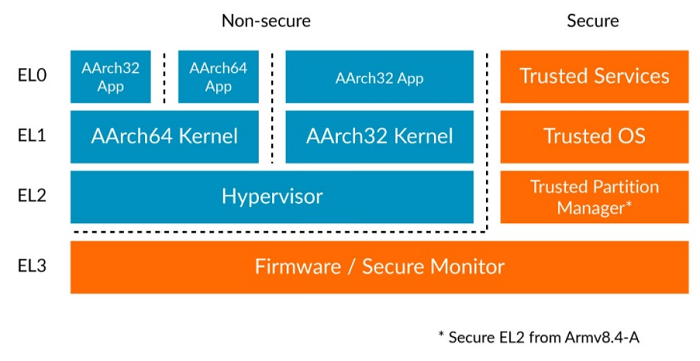
\includegraphics[height=0.75\textheight]{slides/linux-bootloaders-tf-a/arm-exception-levels.png}
  \end{center}
  Source: \href{https://developer.arm.com/documentation/102412/0102/Execution-and-Security-states}{ARM documentation}
\end{frame}

\begin{frame}{Interfaces with secure firmware}
  \begin{columns}
    \column{0.8\textwidth}
    \begin{itemize}
    \item Standardized by ARM
    \item Services
      \begin{itemize}
      \item implemented by the secure firmware
      \item called by the operating system
      \end{itemize}
    \item Prevents the operating system running in normal world from
      directly accessing critical hardware resources
    \item
      \href{http://infocenter.arm.com/help/topic/com.arm.doc.den0022d/Power_State_Coordination_Interface_PDD_v1_1_DEN0022D.pdf}{PSCI},
      Power State Coordination Interface
      \begin{itemize}
      \item Power management related: turn CPUs on/off, CPU idle state,
        platform shutdown/reset
      \end{itemize}
    \item
      \href{http://infocenter.arm.com/help/topic/com.arm.doc.den0056a/DEN0056A_System_Control_and_Management_Interface.pdf}{SCMI},
      System Control and Management Interface
      \begin{itemize}
      \item Power domain, clocks, sensor, performance
      \end{itemize}
    \item Secure firmware implementing these interfaces is
      \begin{itemize}
      \item Mandatory to run Linux on ARMv8
      \item Mandatory to run Linux on some ARMv7 platforms, but not all
      \end{itemize}
    \end{itemize}
    \column{0.2\textwidth}
    \includegraphics[width=\textwidth]{slides/linux-bootloaders-tf-a/arm-interfaces.pdf}
  \end{columns}
\end{frame}

\begin{frame}{TF-A}
  \begin{itemize}
  \item {\em Trusted Firmware-A (TF-A) provides a reference
      implementation of secure world software for Armv7-A and Armv8-A,
      including a Secure Monitor executing at Exception Level 3 (EL3)}
  \item Formerly known as {\em ATF}, for ARM Trusted Firmware
  \item Implements the various standard interfaces that operating
    systems need from the secure firmware
  \item Has drivers for the hardware blocks that are not accessed
    directly by Linux
  \item Needs to be ported for each SoC
  \item Depending on the platform, may also need to be ported per
    board: DDR initialization
  \item Used on the vast majority of ARMv8 platforms, and on a few
    recent ARMv7 platforms
  \item \url{https://www.trustedfirmware.org/projects/tf-a/}
  \end{itemize}
\end{frame}

\begin{frame}{Trusted OS, OP-TEE}
  \begin{itemize}
  \item A trusted operating system can run in the {\em secure world},
    also called {\em Trusted Execution Environment} or {\em TEE}
  \item Hardware partitioning between {\em secure world} and {\em
      normal world}
    \begin{itemize}
    \item Some hardware resources only available in the {\em secure
        world}, by the trusted OS
    \end{itemize}
  \item Allows to run trusted applications/services
    \begin{itemize}
    \item isolated from Linux
    \item can provide services to Linux applications
    \end{itemize}
  \item Most common open-source implementation: {\em OP-TEE}
    \begin{itemize}
    \item Supported by most silicon vendors
    \item \url{https://www.op-tee.org/}
    \end{itemize}
  \end{itemize}
\end{frame}

\begin{frame}{ARM: summary}
  \begin{center}
    \includegraphics[height=0.70\textheight]{slides/linux-bootloaders-tf-a/arm-nomenclature.pdf}
  \end{center}
  {\small Largely inspired from {\em Ahmad Fatoum} presentation
    {\em From Reset Vector to Kernel},
    \href{https://archive.fosdem.org/2021/schedule/event/from_reset_vector_to_kernel/attachments/slides/4632/export/events/attachments/from_reset_vector_to_kernel/slides/4632/from_reset_vector_to_kernel.pdf}{slides},
    \href{https://www.youtube.com/watch?v=-Ak9MWGxd7M}{video}}\\
    See also
    \href{https://trustedfirmware-a.readthedocs.io/en/latest/design/firmware-design.html}
    {details about the ARM terms: BL1, BL2...}
\end{frame}

\begin{frame}{RISC-V}
  \begin{columns}
    \column{0.7\textwidth}
    \begin{itemize}
    \item Linux-class RISC-V processors have several privilege levels
      \begin{itemize}
      \item M-mode: machine mode
      \item S-mode: level at which the Linux kernel runs
      \item U-mode: level at which Linux user-space
        applications run
      \end{itemize}
    \item Some specific HW resources are not accessible in S-mode
    \item A more privileged firmware runs in M-mode
    \item RISC-V has defined SBI, {\em Supervisor Binary Interface}
      \begin{itemize}
      \item Standardized interface between the OS and the firmware
      \item \url{https://github.com/riscv-non-isa/riscv-sbi-doc}
      \end{itemize}
    \item OpenSBI is a reference, open-source implementation of SBI
      \begin{itemize}
      \item \url{https://github.com/riscv-software-src/opensbi}
      \end{itemize}
    \end{itemize}
    \column{0.3\textwidth}
    \includegraphics[width=\textwidth]{slides/linux-bootloaders-tf-a/riscv-boot.pdf}
  \end{columns}
\end{frame}

\subsection{TF-A: Trusted Firmware}

\begin{frame}{Concept of FIP}
  \begin{itemize}
  \item FIP = {\em Firmware Image Package}
  \item Concept specific to TF-A
  \item {\em packaging format used by TF-A to package firmware images
      in a single binary}
  \item Typically used to bundle the BL33, i.e. the U-Boot bootloader
    that will be loaded by TF-A.
  \item \url{https://trustedfirmware-a.readthedocs.io/en/latest/getting_started/tools-build.html}
  \item \url{https://wiki.st.com/stm32mpu/wiki/How_to_configure_TF-A_FIP}
  \end{itemize}
\end{frame}

\begin{frame}{Configuring TF-A}
  \begin{itemize}
  \item TF-A does not use {\em Kconfig} for configuration
  \item All the configuration is based on variables passed on the
    \code{make} command line
  \item Most variables are documented at:
    \url{https://trustedfirmware-a.readthedocs.io/en/latest/getting_started/build-options.html}
  \end{itemize}
\end{frame}

\begin{frame}{Configure TF-A: important variables}
  \begin{itemize}
  \item \code{CROSS_COMPILE}, cross-compiler prefix
  \item \code{ARCH}, CPU architecture: \code{aarch32} or \code{aarch64}
  \item \code{ARM_ARCH_MAJOR}, \code{7} for ARMv7, \code{8} for ARMv8
  \item \code{PLAT}, SoC family, any directory name in \code{plat}
    that contains \code{platform.mk}
  \item \code{AARCH32_SP}, the Secure Payload, specific to
    ARMv7. Either OP-TEE or the built-in {\em SP-MIN} provided by TF-A
  \item \code{DTB_FILE_NAME}, path to the Device Tree describing our board
  \item \code{BL33}, path to the second stage bootloader, usually
    U-Boot, to include in the FIP image
  \item Specific to STM32MP1
    \begin{itemize}
    \item \code{BL33_CFG}, path to the U-Boot Device Tree
    \item \code{STM32MP_SDMMC=1}, enable support for SD card/eMMC in TF-A
    \end{itemize}
  \end{itemize}
\end{frame}

\begin{frame}[fragile]{Building TF-A for STM32MP1}
  \begin{block}{}
    {\footnotesize
\begin{verbatim}
$ make CROSS_COMPILE=arm-linux- \
        ARM_ARCH_MAJOR=7 \
        ARCH=aarch32 \
        PLAT=stm32mp1 \
        AARCH32_SP=sp_min \
        DTB_FILE_NAME=stm32mp157a-dk1.dtb \
        BL33=/path/to/u-boot/u-boot-nodtb.bin \
        BL33_CFG=/path/to/u-boot/u-boot.dtb \
        STM32MP_SDMMC=1 \
        fip all
\end{verbatim}
    }
  \end{block}

  Build results in \code{build/stm32mp1/release}. Important files:

  \begin{itemize}
  \item \code{tf-a-stm32mp157a-dk1.stm32}, TF-A itself
  \item \code{fip.bin}, the FIP image, containing U-Boot and other
    elements
  \end{itemize}
\end{frame}

\begin{frame}[fragile]{FIP image contents}
  \begin{block}{fiptool info}
    {\footnotesize
\begin{verbatim}
$ ./tools/fiptool/fiptool info build/stm32mp1/release/fip.bin
Secure Payload BL32 (Trusted OS): offset=0x100, size=0x8AEC, cmdline="--tos-fw"
Non-Trusted Firmware BL33: offset=0x8BEC, size=0xECE6C, cmdline="--nt-fw"
FW_CONFIG: offset=0xF5A58, size=0x226, cmdline="--fw-config"
HW_CONFIG: offset=0xF5C7E, size=0x16A98, cmdline="--hw-config"
TOS_FW_CONFIG: offset=0x10C716, size=0x3CF6, cmdline="--tos-fw-config"
\end{verbatim}
    }
  \end{block}
\end{frame}

\subsection{Example boot sequences on ARM}

\begin{frame}{STM32MP1: ARMv7}
  \begin{center}
    \includegraphics[width=\textwidth]{slides/linux-bootloaders-tf-a/sequence-stm32mp1.pdf}
  \end{center}
  \vspace{0.3cm}
  Note: booting with U-Boot SPL and U-Boot is also possible.
\end{frame}

\begin{frame}{STM32MP1 partition layout}
  \begin{center}
    \includegraphics[height=0.8\textheight]{slides/linux-bootloaders-tf-a/stm32mp1-tfa.pdf}
  \end{center}
\end{frame}

\begin{frame}{TI AM62x (BeaglePlay): ARMv7 and ARMv8 cores}
  \begin{center}
    \includegraphics[height=0.8\textheight]{slides/linux-bootloaders-tf-a/sequence-am62x.pdf}\\
    \footnotesize See \url{https://u-boot.readthedocs.io/en/latest/board/ti/am62x_sk.html} for details.
  \end{center}
\end{frame}

\begin{frame}{AM62x (BeaglePlay) partition layout}
  \begin{center}
    \includegraphics[height=0.8\textheight]{slides/linux-bootloaders-tf-a/am62x-tfa.pdf}
  \end{center}
\end{frame}

\begin{frame}{TI AM335x (32 bit BeagleBone): ARMv7}
  \begin{center}
    \includegraphics[width=\textwidth]{slides/linux-bootloaders-tf-a/sequence-am335x.pdf}
  \end{center}
\end{frame}

\begin{frame}{NXP i.MX6: ARMv7}
  \begin{center}
    \includegraphics[height=0.7\textheight]{slides/linux-bootloaders-tf-a/sequence-imx.pdf}
  \end{center}
  \vspace{0.1cm}
  Note: this diagram shows one possible boot flow on NXP i.MX6, but it
  is also possible to use the U-Boot SPL $\rightarrow$ U-Boot boot
  flow on i.MX6.
\end{frame}

\begin{frame}{Allwinner ARMv8 cores}
  \begin{center}
    \includegraphics[height=0.8\textheight]{slides/linux-bootloaders-tf-a/sequence-allwinner-64-bit.pdf}
  \end{center}
\end{frame}
